
\chapter{Evaluating the Effects of White Matter Multiple Sclerosis Lesions on the Volume Estimation of 6 Brain Tissue Segmentation
Methods.}  
\label{chapter:chapter_3}
In this chapter, we present an study of the impact of MS white matter lesions on the brain tissue measurements of six well-known segmentation techniques. These include straightforward techniques such as Artificial Neural Network (ANN) and fuzzy C-means (FCM) as well as more advanced techniques such as the Fuzzy And Noise Tolerant Adaptive Segmentation Method (FANTASM), FMRIB's Automated Segmentation Tool (FAST), and Statistical Parametric Mapping (SPM) with versions SPM5 and SPM8. This proposed evaluation has been published in the following paper:

\vspace{2cm}

\noindent\fbox{\parbox[b]{\linewidth}{Paper published in American Journal of Neuroradiology 

Volume: 36, Pages: 1109-1115, Published: February 2015

DOI: 10.3174/ajnr.A4262

Quality Index: 3.59 (Quartile 1)}}
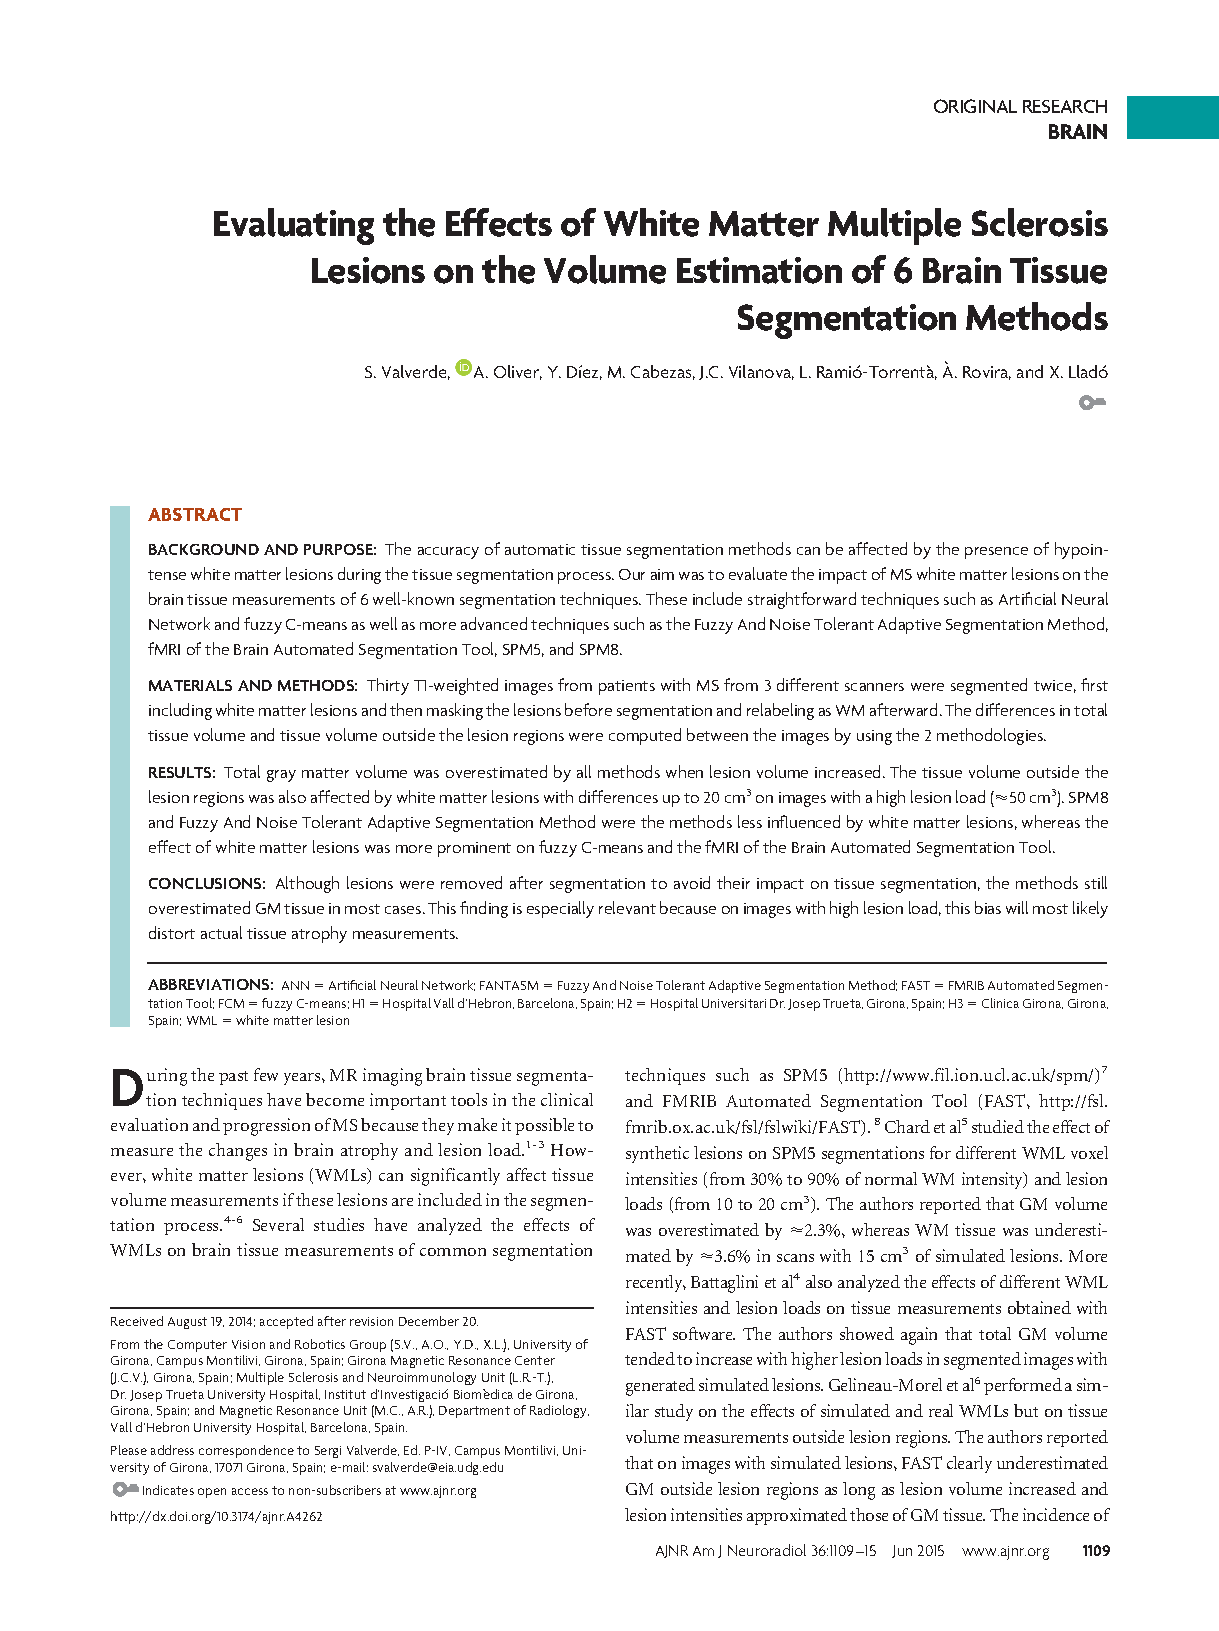
\includepdf[pages={-}]{./papers/ajnr2015.pdf}


%%% Local Variables:
%%% mode: latex
%%% TeX-master: "../main"
%%% End:


